
\documentclass{article}
\usepackage[utf8]{inputenc}
\usepackage{multicol}
\usepackage{amsmath,amsfonts,stmaryrd,amssymb} % Math packages

\usepackage{graphicx, float, subfigure} % Picture package

\usepackage{enumerate} % Custom item numbers for enumerations

\usepackage[ruled]{algorithm2e} % Algorithms

\usepackage[framemethod=tikz]{mdframed} % Allows defining custom boxed/framed environments

\usepackage{listings} % File listings, with syntax highlighting
\lstset{
	basicstyle=\ttfamily, % Typeset listings in monospace font
}

\usepackage{cite}
\usepackage{setspace}

%----------------------------------------------------------------------------------------
%	DOCUMENT MARGINS
%----------------------------------------------------------------------------------------

\usepackage{geometry} % Required for adjusting page dimensions and margins

\geometry{
	paper=a4paper, % Paper size, change to letterpaper for US letter size
	top=2.5cm, % Top margin
	bottom=3cm, % Bottom margin
	left=2.5cm, % Left margin
	right=2.5cm, % Right margin
	headheight=14pt, % Header height
	footskip=1.5cm, % Space from the bottom margin to the baseline of the footer
	headsep=1.2cm, % Space from the top margin to the baseline of the header
	%showframe, % Uncomment to show how the type block is set on the page
}

%----------------------------------------------------------------------------------------
%	FONTS
%----------------------------------------------------------------------------------------

\usepackage[utf8]{inputenc} % Required for inputting international characters
\usepackage[T1]{fontenc} % Output font encoding for international characters

\usepackage{XCharter} % Use the XCharter fonts

 % Include the file specifying the document structure and custom commands
\renewcommand{\baselinestretch}{1.2}

\setcounter{secnumdepth}{4}

\title{Self-adapting Trading Systems Based on Reinforcement Learning} % Title of the assignment


\date{\today} 


\begin{document}

\maketitle % Print the title

\begin{center}
  {\Large Abstract}
%\section*{Abstarct} % Unnumbered section
\end{center}

\noindent This paper aims to build self-adapting trading systems using reinforcement learning techniques in order to maximize the profit. We construct these trading systems by different settings (discounted setting and average-reward setting), control algorithms (SARSA and Q-Learning), reward functions (daily return and Differential Sharpe Ratio) and state spaces. We assume the trader can only take short or long position by a fixed magnitude for the action space. All the systems are simulated on two stock return series and one index return series, and some metrics are used to evaluate their performance in terms of profit and risk. We also set two simple baseline strategies for comparison. The result shows that these trading systems can provide satisfactory profit for regular time series of return, while for irregular and volatile ones they perform poorly most of the time.


\section{Introduction} % Unnumbered section

\noindent The prediction of stock and index returns is always a hot topic in finance. The classic Efficient Market Hypothesis (EMH) states that no investment systems or strategies can consistently yield average returns exceeding the average returns of the market as a whole because the market can instantaneously incorporate all available information into the market prices \cite{pantazopoulos1998financial} \cite{lo2005reconciling}. The assumption underlying this hypothesis is that all participants in the market make decisions completely rationally and always act in their own interest. However, this is usually not the case in real markets especially during the economic downturn. People’s rationality can be affected by a lot of qualities such as overconfidence, risk aversion, group psychology, overreaction and assessment errors \cite{corazza2015q}. According to \cite{bertoluzzo2014reinforcement}, experimental economists have documented several departures of the real investors’ behaviors from the ones prescribed by the EMH since the 80s of the past century. In addition, most approaches applied to testify the EMH are based on linear models which are not capable of identifying dynamic or nonlinear relationships in the historic data. According to \cite{chenoweth1996embedding}, some suitable nonparametric machine learning approaches may be able to discover more complex nonlinear relationships through learning from examples. Actually, more and more works have emerged in recent years focusing on prediction of financial returns using machine learning techniques such as neural networks and some of them really achieved a satisfactory result \cite{pantazopoulos1998financial} \cite{chenoweth1996embedding}.

\indent Given these deficiencies of EMH, Andrew has proposed the Adaptive Markets Hypothesis (AMH) which is an extension of the EMH in \cite{lo2005reconciling}. The AMH states that the market is not always efficient and the efficiency degree depends on factors such as number of participants, adaptation ability of participants and the available profit opportunities. It indicates that investors often make mistakes or irrational decisions but they can learn and adapt their behavior in the everchanging market \cite{corazza2015q}. In this context, trading strategies implemented by reinforcement learning (RL) algorithms may lead to satisfactory profit since it can adapt to new information quickly by self-learning. As introduced in \cite{sutton2018reinforcement}, the basic mechanism of RL is that the agent learns what to do by interacting with the environment so as to maximize a numerical reward signal. In contrast with supervised learning methods, RL methods do not require labelled training data as input and can real-time adjust the model according to new information. In this paper, we build a trading system based on reinforcement learning using two algorithms belonging to RL: SARSA and Q-Learning. We also try different settings and reward functions, and compare the final profit with that of two simple baseline strategies: trend following and mean reversion. We test our trading systems using two stock daily return series (Apple Inc. stock and SunPower Corp. stock) and one index daily return series (S\&P 500 Index). All methods discussed in this paper does not take the transaction cost into account.

\section{Methodology}

\subsection{Problem Formulation} % Unnumbered section

\noindent The goal of our trading system is to maximize the final profit by choose which position to take on each day, so the action space contains all the possible positions the trader can take in the problem. This paper assumes that the trader can only take short or long position by a fixed magnitude as follows:

% Math equation/formula
\begin{equation}
	A_{t} \in \left \{ -1, 1 \right \}
\end{equation}

\noindent Here -1 represents taking short position, 1 represents taking long position and $t$ is the business day of the exchange. This action space corresponds to the reversal trading strategy which allows no neutral state (the trader temporarily be out the market by taking no position) \cite{moody1998performance}. The state space is dependent on the length of return window ($K$) we select for the system. The space consists of the most recent $K$ daily returns and the last performed action \cite{corazza2015q}, which is described as follows:

% Math equation/formula
\begin{equation}
	S_{t} = \left [ r_{t-K+1},...,r_{t}, A_{t-1} \right ]
\end{equation}

\noindent Here $r_{t}$ represents the stock or index log return on day $t$ defined as $r_{t} = ln\left ( p_{t}/p_{t-1} \right )$ where $p_{t}$ is the stock or index price on day $t$. For example, if $K = 5$, the state on each day is composed of returns of the last four days, today's return and the last performed action. Therefore, the larger $K$ is, the trading system contains more memory and the action taken by the system depends on longer window of history returns. In this paper, we test the trading system with $K$ from 1 to 5 for all the methods.

\indent To approximate the action-state value $q\left ( S_{t}, A_{t} \right )$, we apply the linear function of a weight vector $\mathbf{w}$. The approximation formula is 

% Math equation/formula
\begin{equation}
	\hat{q}\left ( S_{t}, A_{t}, \mathbf{w}_{t} \right ) = w_{t,0}+\sum_{i=1}^{K}w_{t,i}r_{t-K+i} + w_{t,K+1}A_{t-1} +w_{t,K+2}A_{t}
\end{equation}

\noindent where $\hat{q}\left ( S_{t}, A_{t}, \mathbf{w}_{t} \right )$ is the approximation of the true value $q\left ( S_{t}, A_{t} \right )$. Note here the feature values of the state-action pair are simply all the components in today's state space plus today's action value. To update the weight vector day by day, we apply the semi-gradient method in order to minimize the mean square error between $q\left ( S_{t}, A_{t} \right )$ and $\hat{q}\left ( S_{t}, A_{t}, \mathbf{w}_{t} \right )$ \cite{sutton2018reinforcement}. The general update rule is as follows:

% Math equation/formula
\begin{equation}
	\mathbf{w}_{t+1} = \mathbf{w}_{t}+\alpha \left [ q\left ( S_{t}, A_{t} \right )-\hat{q}\left ( S_{t}, A_{t}, \mathbf{w}_{t} \right ) \right ]\mathbf{x}\left ( S_{t}, A_{t} \right )
\end{equation}

\noindent where $\alpha$ is the learning rate and $\mathbf{x}\left ( S_{t}, A_{t} \right )$ is the feature vector defined as 

% Math equation/formula
\begin{equation}
	\mathbf{x}\left ( S_{t}, A_{t} \right ) = \left ( 1, r_{t-K+1},..., r_{t}, A_{t-1}, A_{t} \right )^{T}.
\end{equation}

\noindent Note that we set the initial value of the weight vector as the zero vector for all methods.

\indent In equation (4), $q\left ( S_{t}, A_{t} \right )$ is the true action-state value that we do not know, thus we need to some approximation for it to implement the update. In the following sections, we will introduce different settings and algorithms that apply different approximations for the true action-state value. 

\subsection{Problem Setting} % Unnumbered section

\noindent Theoretically, a trader can trade eternally in the financial market without getting out of it. Therefore the trading system we aim to build in this paper is actually a continuing task. As introduced in \cite{sutton2018reinforcement}, there are two settings suitable for dealing with continuing problems: discounted setting and average-reward setting.

\indent In discounted setting, the sum of rewards the agent tries to maximize is defined as follows:

% Math equation/formula
\begin{equation}
	G_{t}^{d} = R_{t+1}+\gamma R_{t+2}+\gamma ^{2} R_{t+3}+\cdot \cdot \cdot =\sum_{i=0}^{\infty }\gamma ^{i}R_{t+i+1}
\end{equation}

\noindent where $R_{t+1}$ is the reward obtained on day $t+1$ after taking $A_{t}$ on day $t$ and $\gamma$ is the discount rate between 0 and 1. As $\gamma$ approaches 1, the value of future rewards added to $G_{t}$ becomes larger and the agent becomes more farsighted.

\indent In average-reward setting, we use a different formula for the sum of reward on day $t$:

% Math equation/formula
\begin{equation}
	G_{t}^{c} = R_{t+1}-r\left ( \pi  \right )+R_{t+2}-r\left ( \pi  \right )+R_{t+3}-r\left ( \pi  \right )+\cdot \cdot \cdot 
\end{equation}

\noindent Here $r\left ( \pi  \right )$ is the average reward of policy $\pi$ defined by the following equation:

% Math equation/formula
\begin{equation}
	r\left ( \pi  \right ) = \lim_{h\rightarrow \infty }\frac{1}{h}\sum_{t=1}^{h}\mathbb{E}\left [ R_{t} \mid S_{0} ,A_{0:t-1}\sim \pi \right ]
\end{equation}

\noindent where $S_{0}$ is the initial state and $A_{0:t-1}$ is all the actions from day $0$ to day $t-1$ generated by the policy $\pi$. Note that the average reward $r\left ( \pi  \right )$ is actually a true value that we do not know, however, some approximations which will be discussed in the next section can be derived to substitute it in the algorithm. 

\indent The two settings are both applied for continuing problems but with different implication. The discounted setting emphasizes more on the instant reward while the average-reward setting pays as much attention to the future rewards as to the instant one. This paper applies both settings with different control algorithms and different reward functions, testing all the trading systems on the three different return time series for comparison.


\subsection{Control Algorithm} % Unnumbered section


\noindent In this paper, we consider two online temporal-difference algorithms learning the optimal action-state value $q^{\ast }\left ( S_{t}, A_{t} \right )$ : SARSA and Q-Learning. The most important difference between the two algorithms is that SARSA is an on-policy method which updates the action-state value in line with the policy it follows while Q-Learning is an off-policy method which updates the action-state value on the basis of the greedy policy that always selects the action with the maximum action value. This paper employs the $\epsilon$-greedy policy with $\epsilon = 0.1$ to generate the actions on each day for all the algorithms.


\indent In the discounted setting, the weight vector updating formulas for both SARSA and Q-Learning algorithms can be derived respectively as equation (9) and (10):

% Math equation/formula
\begin{equation}
	\mathbf{w}_{t+1} = \mathbf{w}_{t}+\alpha \left [ R_{t+1}+\gamma \hat{q}\left ( S_{t+1}, A_{t+1}, \mathbf{w}_{t} \right ) -\hat{q}\left ( S_{t}, A_{t}, \mathbf{w}_{t} \right ) \right ]\mathbf{x}\left ( S_{t}, A_{t} \right )
\end{equation}

% Math equation/formula
\begin{equation}
	\mathbf{w}_{t+1} = \mathbf{w}_{t}+\alpha \left [ R_{t+1}+\gamma \max_{A_{t+1}}\hat{q}\left ( S_{t+1}, A_{t+1}, \mathbf{w}_{t} \right ) -\hat{q}\left ( S_{t}, A_{t}, \mathbf{w}_{t} \right ) \right ]\mathbf{x}\left ( S_{t}, A_{t} \right )
\end{equation}

\indent In the average-reward setting, the update formulas for both algorithms can be derived similarly by just changing the approximation for the true action-state value:

% Math equation/formula
\begin{equation}
	\mathbf{w}_{t+1} = \mathbf{w}_{t}+\alpha \left [ R_{t+1}-\bar{R_{t}}+\hat{q}\left ( S_{t+1}, A_{t+1}, \mathbf{w}_{t} \right ) -\hat{q}\left ( S_{t}, A_{t}, \mathbf{w}_{t} \right ) \right ]\mathbf{x}\left ( S_{t}, A_{t} \right )
\end{equation}

% Math equation/formula
\begin{equation}
	\mathbf{w}_{t+1} = \mathbf{w}_{t}+\alpha \left [ R_{t+1}-\bar{R_{t}}+\max_{A_{t+1}}\hat{q}\left ( S_{t+1}, A_{t+1}, \mathbf{w}_{t} \right ) -\hat{q}\left ( S_{t}, A_{t}, \mathbf{w}_{t} \right ) \right ]\mathbf{x}\left ( S_{t}, A_{t} \right )
\end{equation}

\noindent Here $\bar{R_{t}}$ is an estimate of the average reward $r\left ( \pi  \right )$ on day $t$. For each algorithm, we update the estimation day by day using the following formulas respectively:

% Math equation/formula
\begin{equation}
	\bar{R_{t+1}} = \bar{R_{t}}+\beta \left [ R_{t+1}-\bar{R_{t}}+\hat{q}\left ( S_{t+1}, A_{t+1}, \mathbf{w}_{t} \right ) -\hat{q}\left ( S_{t}, A_{t}, \mathbf{w}_{t} \right ) \right ]
\end{equation}


% Math equation/formula
\begin{equation}
	\bar{R_{t+1}} = \bar{R_{t}}+\beta \left [ R_{t+1}-\bar{R_{t}}+\max_{A_{t+1}}\hat{q}\left ( S_{t+1}, A_{t+1}, \mathbf{w}_{t} \right ) -\hat{q}\left ( S_{t}, A_{t}, \mathbf{w}_{t} \right ) \right ]
\end{equation}

\noindent where $\beta$ is another learning rate independent of $\alpha$.

\indent We can see the update formulas for both settings and both algorithms are very similar to equation (4) except that they use different approximations to substitute the true action-state value $q\left ( S_{t}, A_{t} \right )$. Therefore, the only difference between these four algorithms is about how we choose the representation for the true action-state value that we want to approximate.

\subsection{Reward Function} % Unnumbered section

\noindent Up to now, we have not defined the reward of the problem $R_{t}$. This paper applies two ways to calculate the reward. The first way is quite straightforward, that is taking the obtained return on day $t$ as the reward. The formula definition is as follows:

% Math equation/formula
\begin{equation}
	R_{t}^{r} = A_{t-1}r_{t}
\end{equation}

\indent In the second way we take the Differential Sharpe Ratio (DSR) proposed in \cite{moody1998performance} as our reward. We define it with the formulas below:

% Math equation/formula
\begin{equation}
	a_{t} = a_{t-1} + \eta \Delta a_{t}= a_{t-1}+\eta \left ( R_{t}^{r}-a_{t-1} \right )
\end{equation}

% Math equation/formula
\begin{equation}
	b_{t} = b_{t-1} + \eta \Delta b_{t}= b_{t-1}+\eta \left ( (R_{t}^{r})^{2}-b_{t-1} \right )
\end{equation}

% Math equation/formula
\begin{equation}
	R_{t}^{dsr} = D_{t} = \frac{b_{t-1}\Delta a_{t}-\frac{1}{2}a_{t-1}\Delta b_{t}}{\left ( b_{t-1}-a_{t-1}^{2} \right )^{3/2}}
\end{equation}

\noindent where $a_{t}$ and $b_{t}$ are exponential moving estimates of the first and second moments of Sharpe Ratio respectively with $a_{0} = b_{0} = 0$. Note here $\eta$ is another learning rate independent of $\alpha$ and $\beta$. The main advantage of applying DSR instead of directly using Sharpe Ratio as the reward is that it can be computed incrementally and thus much more efficiently as we do not need to recompute the average and standard deviation of obtained returns for the entire trading history in order to update the Sharpe Ratio for the most recent time period. In addition, in DSR recent returns receive more weightings than older ones, while in Sharpe Ratio all returns are treated equally \cite{moody1998performance}.

\indent With DSR as the reward function, there is a little problem that we cannot obtain the value of $R_{1}^{dsr}$ since $a_{0}$ and $b_{0}$ are all 0. One way to solve it is that we use $R_{1}^{r}$ to replace $R_{1}^{dsr}$ for the first day and calculate $R_{t}^{dsr}$ when $t > 1$.

\section{Financial Data} % Unnumbered section

\noindent In order to test the performance of our trading systems, we select two stock daily return time series and one index daily return time series. The two stocks are Apple Inc. stock (AAPL) and SunPower Corp. stock (SPWR) whose adjusted close prices can be downloaded from Yahoo Finance (https://finance.yahoo.com/). For AAPL we choose the time series from 2000-01-03 to 2021-04-23 with 5361 daily price data in total and for SPWR we choose the time series from 2005-11-18 to 2021-04-23 with 3882 daily price data in total. The index we choose is S\&P 500 Index (S\&P500) whose close prices can be downloaded from https://info.bossa.pl/pub/metastock/indzagr/mstzgr.zip . For S\&P 500 we select the window from 2000-01-03 to 2021-01-29 with 5302 daily price data. After checking the data we do not find any obvious outlier or abnormity, hence we just trust in the original data.

\section{Baseline Strategy} % Unnumbered section

\noindent To test if the trading systems based on reinforcement learning algorithms can somehow capture the complexity in financial data, we also run two simple trading strategies which can be regarded as baseline strategies for comparison. The two strategies take actions only according to today's return: if the return is positive, the first strategy takes long position while the second one takes short position, and vise versa. We can formulate the two strategies by following equations:

% Math equation/formula
\begin{equation}
	A_{t}^{tf} = sign(r_{t})
\end{equation}

% Math equation/formula
\begin{equation}
	A_{t}^{mr} = -sign(r_{t})
\end{equation}

\noindent Basically we can think of them as the most simplified ones of trend following strategies and mean reversion strategies respectively.

\section{Empirical Result} % Unnumbered section

\noindent We evaluate the performance of our trading systems constructed as above by simulating trading on the three time series returns. That is, given a certain amount of initial money, the system takes actions (long or short all the current capital) generated from the $\epsilon$-greedy policy every day, and the obtained daily profit (or loss) is recorded and added to (or deducted from) the current capital for the trading on next day. The whole process continues until we run out of time series data. 
\indent In the methodology section we have introduced two settings (discounted setting and continuing setting), two algorithms (SARSA and Q-Learning), two reward functions (obtained return and Differential Sharpe Ratio) and five $K$ values ($K$ from 1 to 5), therefore by combining them in different ways we can get 40 different trading systems in total. For each trading system we do 100 simulations on the three times series data respectively and summarize the final result. As for the hyperparameter setting, we choose $\alpha = \beta = \eta = 0.05$, $\gamma = 0.95$ and $\epsilon = 0.1$ for all systems.


% Picture insertion
\begin{figure}[H]
	\centering
	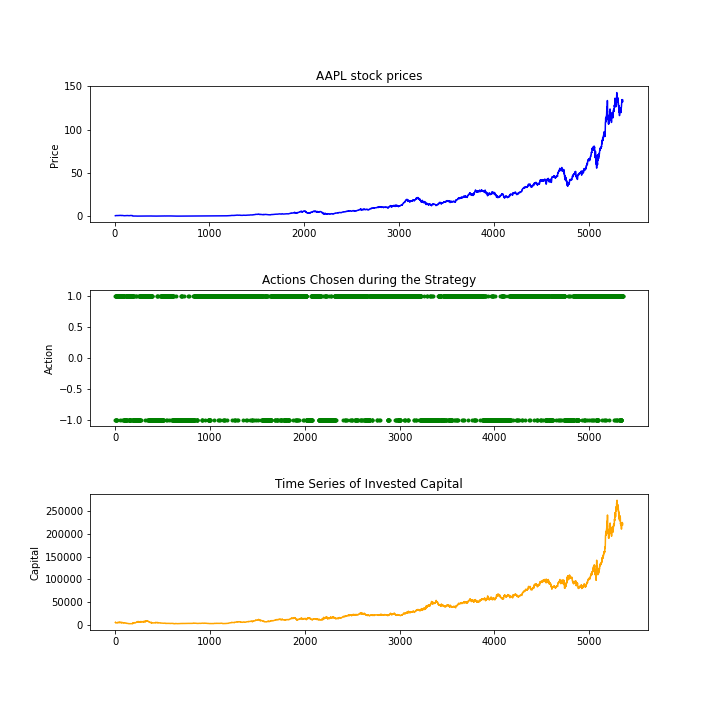
\includegraphics[scale=0.4]{figs/figure1.png}
	\caption{One simulation result with discounted setting, daily obtained return and SARSA with $K = 5$, initial investment $= 5000$ on AAPL} 
	\label{figure1}
\end{figure}




% Picture insertion
\begin{figure}[H]
	\centering
	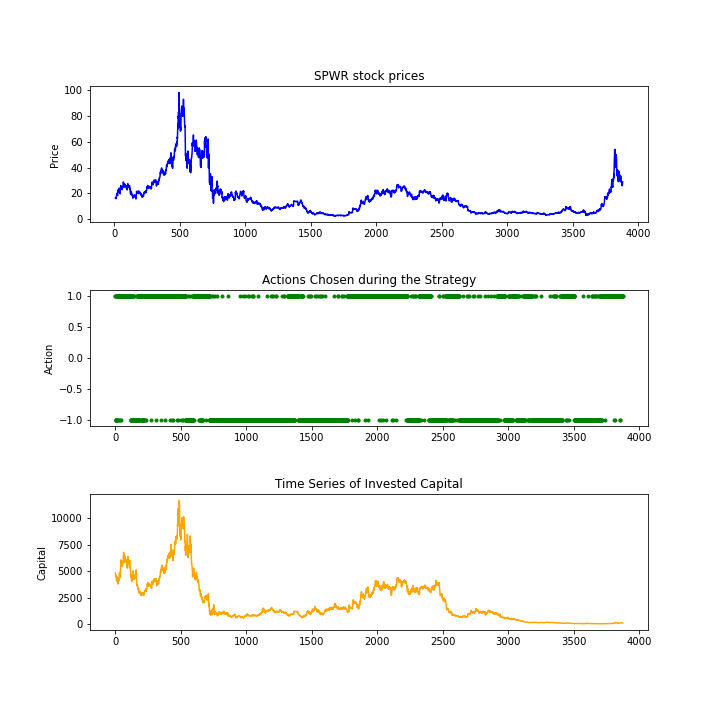
\includegraphics[scale=0.4]{figs/figure2.png}
	\caption{One simulation result with discounted setting, daily obtained return and SARSA with $K = 5$, initial investment $= 5000$ on SPWR} 
	\label{figure2}
\end{figure}

\indent Figure 1 shows some detailed information for a particular simulation conducted by the system using discounted setting, daily obtained return and SARSA algorithm with $K = 5$ on the AAPL stock returns. The initial investment is set to 5000 in this simulation. We can see the time series of stock price is similar to that of the capital in the system, indicating the system takes long position most of the time. The second plot verifies it since the dots above are denser than those below. The final profit for this simulation is 215405.84, about 43 times the initial investment. Actually, this amount of profit is much larger than the profit achieved by taking the long position all the time (89584.41).


\indent Figure 2 displays the detailed result for a simulation implemented by the same system but on the SPWR stock returns with the same initial investment 5000. The price time series of SPWR seems to be more random and volatile than that of AAPL, as a result the system performs bad with a negative final profit (-4900.60). 

\indent We put all the summarized simulation results in Table 1 - 24 (in Appendix), each one contains the performance of systems with a single combination of different settings, algorithms and rewards. The metrics we use to measure the performance include the mean and standard deviation of final returns, 95\% empirical Value at Risk (VaR) and Expected Shortfall (ES), and the proportion of days with positive return. The performances differ on different time series data.

\indent For AAPL stock returns, the systems with discounted setting and daily return reward distinctly outperform the other ones since they produce much higher final returns (Table 1 and 2). The 95\% empirical VaR and ES of them are also satisfactory and some VaR's are even positive, meaning we have less then 5\% chance to lose money. For the two kinds of systems in Table 1 and 2, we can also see the difference between SARSA and Q-Learning algorithms are not obvious and both of them achieve the highest final return when $K = 3$. For other kinds of systems (Table 3 - 8), they all produce positive final returns, though much lower than the first two. In addition, the proportions of days with positive return achieved by all the systems on AAPL are bigger than 50\%



\indent For SPWR almost all the systems provide negative final returns meaning we will lose money at last. The systems with average-reward setting and daily return reward seem to perform slightly better than others since they get some chances to make money at last (Table 11 and 12). The proportions of days with positive return for all systems are below 50\%, that might explains some of the reasons why the systems perform much worse on SPWR than on AAPL.






\indent Like the results on AAPL, the performance of systems differ largely on S\&P 500 index. Clearly, the systems with discounted setting and daily return reward beat the others again 
with respect to final profit and risk measures (Table 17 and 18). Note that only these two kinds of systems provide positive final returns while the others produce negatives ones. The difference between SARSA and Q-Learning is still not apparent and for the two kinds of systems in Table 17 and 18, systems with $K = 2$ or $K = 3$ appear to be slightly better than others. Besides, with respect to the proportion of days obtaining positive return, the systems with daily return reward clearly outperform those with DSR reward since the values of former ones are all above 50\% while the values of latter ones are all below 50\%.



\indent Table 25 (in Appendix) shows the result obtained by our two baseline strategies. The simple trend following strategy performs terribly on all three stock and index returns. Our trading systems can beat it at least on AAPL and S\&P500. The mean reversion strategy also performs poorly on AAPL and SPWR, however, it acts surprisingly well on S\&P500 with final return as high as 1500\%, so much better than our best trading system on the S\&P 500 index.




\section{Conclusion} % Unnumbered section

\noindent In this paper, we build 40 trading systems with different combinations of settings, algorithms, reward functions and $K$ values based on reinforcement learning techniques. We test their performances on three return time series: AAPL, SPWR and S\&P500 by simulation. Two simple baseline strategies are also implemented for comparison.


\indent The simulation result illustrates that performance of the trading systems mainly depends on which stock or index return they perform on. Different return time series might lead to quite different final profits. For the choice of reward function, daily return reward seems to be more suitable for this problem than DSR reward since the systems with it can produce better result. The performances of SARSA and Q-Learning are often very similar, although in theory Q-Learning cannot converge to the target in the linear approximation case. With regard to the problem settings and $K$ values, we cannot get much information from the result, indicating the choices of them might be problem-specific. For example, systems with discounted setting and daily return reward perform best on AAPL and S\&P500 while those with average-reward setting and daily return reward seem to be relatively superior in the case of SPWR. Compared with the two baseline strategies, our trading systems can beat them most of the time with only one exception: the simple mean reversion strategy on S\&P 500 index.

\indent To conclude, there is no one single system that can always provide the trader satisfactory profit on any stock or index. For return series with some regular patterns like AAPL, trading systems based on RL can successfully capture the pattern and produce quite considerable profit. However, for return series which are volatie and contain a lot of randomness like SPWR, RL may fail to learn the potential trend inside and perform badly.


\section{Reflection and Further Research} % Unnumbered section

\noindent Here I point out three main directions future researches may focus on: transaction cost, feature construction and policy gradient methods.

\indent First, this paper assumes no transaction cost for trading, which is not the case in reality. The addition of transaction cost in trading systems might somehow prevent the trader from trading frequently and produce new interesting result.

\indent Second, we apply a very simple feature construction in this paper where the feature vector involves last $K$ days' returns and two actions. Actually we also try some transformations of the features but they perform even worse (ex. taking the sign of return or normalizing the return). Further works may apply more advanced approaches to construct the feature vector.

\indent Finally, the methods applied in this paper all belong to
so-called action-value methods \cite{sutton2018reinforcement}, that is we estimate the action-state values and choose actions based on them. However, policy gradient methods can directly learn a parameterized policy which selects actions without consulting the action values. Several advantages of it over the action-value methods are explained in \cite{sutton2018reinforcement}. Actually, this type of methods has become popular in RL recently and should be considered in further research.

\clearpage

\bibliographystyle{plain}   
\bibliography{references}  % Reference




\section*{Appendix} % Unnumbered section

\begin{table}[H]
\centering
\begin{tabular}{|l|r|r|r|r|r|} 
\hline
                             & \multicolumn{1}{l|}{K = 1} & \multicolumn{1}{l|}{K = 2} & \multicolumn{1}{l|}{K = 3} & \multicolumn{1}{l|}{K = 4} & \multicolumn{1}{l|}{K = 5}  \\ 
\hline
Mean of final returns        & 43.4050                    & 39.8486                    & 51.0859                    & 25.0588                    & 27.9842                     \\ 
\hline
SD of final returns          & 86.6321                    & 66.0739                    & 75.9887                    & 30.8852                    & 47.6678                     \\ 
\hline
95\% VaR                     & -0.1959                    & 0.2433                     & 0.0401                     & -0.1851                    & -0.1972                     \\ 
\hline
95\% ES                      & -0.2990                    & -0.1519                    & -0.4150                    & -0.4896                    & -0.6748                     \\ 
\hline
Days of positive return (\%) & 0.5199                     & 0.5194                     & 0.5194                     & 0.5184                     & 0.5193                      \\
\hline
\end{tabular}
\caption{Simulation result with discounted setting, daily return reward and SARSA on AAPL}
\label{table1}
\end{table}


\begin{table}[H]
\centering
\begin{tabular}{|l|r|r|r|r|r|} 
\hline
                             & \multicolumn{1}{l|}{K = 1} & \multicolumn{1}{l|}{K = 2} & \multicolumn{1}{l|}{K = 3} & \multicolumn{1}{l|}{K = 4} & \multicolumn{1}{l|}{K = 5}  \\ 
\hline
Mean of final returns        & 29.7910                    & 38.8263                    & 42.7774                    & 30.8733                    & 32.1441                     \\ 
\hline
SD of final returns          & 42.6141                    & 44.4653                    & 91.7654                    & 41.0633                    & 70.8737                     \\ 
\hline
95\% VaR                     & 0.0188                     & 0.3646                     & 0.6562                     & 0.2358                     & -0.4775                     \\ 
\hline
95\% ES                      & -0.2648                    & -0.0944                    & 0.3783                     & 0.1178                     & -0.6836                     \\ 
\hline
Days of positive return (\%) & 0.5201                     & 0.5207                     & 0.5199                     & 0.5205                     & 0.5202                      \\
\hline
\end{tabular}
\caption{Simulation result with discounted setting, daily return reward and Q-learning on AAPL}
\label{table2}
\end{table}

\begin{table}[H]
\centering
\begin{tabular}{|l|r|r|r|r|r|} 
\hline
                             & \multicolumn{1}{l|}{K = 1} & \multicolumn{1}{l|}{K = 2} & \multicolumn{1}{l|}{K = 3} & \multicolumn{1}{l|}{K = 4} & \multicolumn{1}{l|}{K = 5}  \\ 
\hline
Mean of final returns        & 9.6824                     & 5.7349                     & 7.6947                     & 7.5099                     & 4.2008                      \\ 
\hline
SD of final returns          & 33.1354                    & 13.9487                    & 25.7142                    & 15.9895                    & 10.5129                     \\ 
\hline
95\% VaR                     & -0.9732                    & -0.9313                    & -0.8573                    & -0.9357                    & -0.8755                     \\ 
\hline
95\% ES                      & -0.9816                    & -0.9447                    & -0.9129                    & -0.9621                    & -0.9199                     \\ 
\hline
Days of positive return (\%) & 0.5102                     & 0.5094                     & 0.5108                     & 0.5096                     & 0.5096                      \\
\hline
\end{tabular}
\caption{Simulation result with average-reward setting, daily return reward and SARSA on AAPL}
\label{table3}
\end{table}

\begin{table}[H]
\centering
\begin{tabular}{|l|r|r|r|r|r|} 
\hline
                             & \multicolumn{1}{l|}{K = 1} & \multicolumn{1}{l|}{K = 2} & \multicolumn{1}{l|}{K = 3} & \multicolumn{1}{l|}{K = 4} & \multicolumn{1}{l|}{K = 5}  \\ 
\hline
Mean of final returns        & 12.3541                    & 4.6959                     & 9.0272                     & 8.1801                     & 5.2103                      \\ 
\hline
SD of final returns          & 47.3607                    & 10.6387                    & 20.3427                    & 26.5924                    & 13.2134                     \\ 
\hline
95\% VaR                     & -0.8342                    & -0.9486                    & -0.9334                    & -0.8784                    & -0.9678                     \\ 
\hline
95\% ES                      & -0.8840                    & -0.9659                    & -0.9540                    & -0.9439                    & -0.9732                     \\ 
\hline
Days of positive return (\%) & 0.5107                     & 0.5094                     & 0.5099                     & 0.5098                     & 0.5107                      \\
\hline
\end{tabular}
\caption{Simulation result with average-reward setting, daily return reward and Q-learning on AAPL}
\label{table4}
\end{table}

\begin{table}[H]
\centering
\begin{tabular}{|l|r|r|r|r|r|} 
\hline
                             & \multicolumn{1}{l|}{K = 1} & \multicolumn{1}{l|}{K = 2} & \multicolumn{1}{l|}{K = 3} & \multicolumn{1}{l|}{K = 4} & \multicolumn{1}{l|}{K = 5}  \\ 
\hline
Mean of final returns        & 3.1406                     & 7.0823                     & 4.7546                     & 7.2004                     & 2.1347                      \\ 
\hline
SD of final returns          & 7.1130                     & 26.7865                    & 19.5442                    & 40.9371                    & 5.2376                      \\ 
\hline
95\% VaR                     & -0.9201                    & -0.9006                    & -0.9520                    & -0.9472                    & -0.9799                     \\ 
\hline
95\% ES                      & -0.9378                    & -0.9257                    & -0.9673                    & -0.9590                    & -0.9892                     \\ 
\hline
Days of positive return (\%) & 0.5091                     & 0.5082                     & 0.5079                     & 0.5076                     & 0.5090                      \\
\hline
\end{tabular}
\caption{Simulation result with discounted setting, DSR reward and SARSA on AAPL}
\label{table5}
\end{table}

\begin{table}[H]
\centering
\begin{tabular}{|l|r|r|r|r|r|} 
\hline
                             & \multicolumn{1}{l|}{K = 1} & \multicolumn{1}{l|}{K = 2} & \multicolumn{1}{l|}{K = 3} & \multicolumn{1}{l|}{K = 4} & \multicolumn{1}{l|}{K = 5}  \\ 
\hline
Mean of final returns        & 7.0499                     & 6.5861                     & 3.4722                     & 7.1611                     & 7.2469                      \\ 
\hline
SD of final returns          & 15.9684                    & 10.7367                    & 10.4000                    & 16.6565                    & 21.4337                     \\ 
\hline
95\% VaR                     & -0.7659                    & -0.7636                    & -0.9295                    & -0.9689                    & -0.8997                     \\ 
\hline
95\% ES                      & -0.8395                    & -0.8193                    & -0.9616                    & -0.9743                    & -0.9385                     \\ 
\hline
Days of positive return (\%) & 0.5110                     & 0.5111                     & 0.5099                     & 0.5105                     & 0.5100                      \\
\hline
\end{tabular}
\caption{Simulation result with discounted setting, DSR reward and Q-learning on AAPL}
\label{table6}
\end{table}

\begin{table}[H]
\centering
\begin{tabular}{|l|r|r|r|r|r|} 
\hline
                             & \multicolumn{1}{l|}{K = 1} & \multicolumn{1}{l|}{K = 2} & \multicolumn{1}{l|}{K = 3} & \multicolumn{1}{l|}{K = 4} & \multicolumn{1}{l|}{K = 5}  \\ 
\hline
Mean of final returns        & 2.8839                     & 3.2694                     & 3.3881                     & 0.6956                     & 0.5849                      \\ 
\hline
SD of final returns          & 11.0922                    & 15.9100                    & 10.0878                    & 3.8710                     & 3.1052                      \\ 
\hline
95\% VaR                     & -0.9868                    & -0.9454                    & -0.9893                    & -0.9819                    & -0.9875                     \\ 
\hline
95\% ES                      & -0.9925                    & -0.9773                    & -0.9901                    & -0.9860                    & -0.9923                     \\ 
\hline
Days of positive return (\%) & 0.5056                     & 0.5063                     & 0.5058                     & 0.5043                     & 0.5041                      \\
\hline
\end{tabular}
\caption{Simulation result with average-reward setting, DSR reward and SARSA on AAPL}
\label{table7}
\end{table}

\begin{table}[H]
\centering
\begin{tabular}{|l|r|r|r|r|r|} 
\hline
                             & \multicolumn{1}{l|}{K = 1} & \multicolumn{1}{l|}{K = 2} & \multicolumn{1}{l|}{K = 3} & \multicolumn{1}{l|}{K = 4} & \multicolumn{1}{l|}{K = 5}  \\ 
\hline
Mean of final returns        & 1.9912                     & 8.5075                     & 1.8761                     & 0.3844                     & 1.5754                      \\ 
\hline
SD of final returns          & 10.2180                    & 21.0031                    & 5.3173                     & 3.1959                     & 4.7470                      \\ 
\hline
95\% VaR                     & -0.9753                    & -0.9233                    & -0.9805                    & -0.9875                    & -0.9863                     \\ 
\hline
95\% ES                      & -0.9867                    & -0.9505                    & -0.9880                    & -0.9905                    & -0.9918                     \\ 
\hline
Days of positive return (\%) & 0.5054                     & 0.5075                     & 0.5054                     & 0.5040                     & 0.5037                      \\
\hline
\end{tabular}
\caption{Simulation result with average-reward setting, DSR reward and Q-learning on AAPL}
\label{table8}
\end{table}

% ----------------------------------------------------------------------------------------------------------------------------------------------------------------------------------------------------

\begin{table}[H]
\centering
\begin{tabular}{|l|r|r|r|r|r|} 
\hline
                             & \multicolumn{1}{l|}{K = 1} & \multicolumn{1}{l|}{K = 2} & \multicolumn{1}{l|}{K = 3} & \multicolumn{1}{l|}{K = 4} & \multicolumn{1}{l|}{K = 5}  \\ 
\hline
Mean of final returns        & -0.5368                    & -0.2998                    & -0.3464                    & -0.3327                    & -0.4270                     \\ 
\hline
SD of final returns          & 0.8350                     & 1.3931                     & 2.4811                     & 2.1848                     & 0.9438                      \\ 
\hline
95\% VaR                     & -0.9939                    & -0.9953                    & -0.9940                    & -0.9984                    & -0.9950                     \\ 
\hline
95\% ES                      & -0.9959                    & -0.9973                    & -0.9967                    & -0.9990                    & -0.9966                     \\ 
\hline
Days of positive return (\%) & 0.4989                     & 0.4991                     & 0.4990                     & 0.4990                     & 0.4995                      \\
\hline
\end{tabular}
\caption{Simulation result with discounted setting, daily return reward and SARSA on SPWR}
\label{table9}
\end{table}

\begin{table}[H]
\centering
\begin{tabular}{|l|r|r|r|r|r|} 
\hline
                             & \multicolumn{1}{l|}{K = 1} & \multicolumn{1}{l|}{K = 2} & \multicolumn{1}{l|}{K = 3} & \multicolumn{1}{l|}{K = 4} & \multicolumn{1}{l|}{K = 5}  \\ 
\hline
Mean of final returns        & -0.6953                    & -0.3093                    & -0.2271                    & -0.6167                    & -0.3872                     \\ 
\hline
SD of final returns          & 0.6337                     & 2.2766                     & 2.0395                     & 0.9143                     & 1.2334                      \\ 
\hline
95\% VaR                     & -0.9966                    & -0.9922                    & -0.9919                    & -0.9976                    & -0.9973                     \\ 
\hline
95\% ES                      & -0.9978                    & -0.9952                    & -0.9968                    & -0.9989                    & -0.9987                     \\ 
\hline
Days of positive return (\%) & 0.4974                     & 0.4991                     & 0.4974                     & 0.4978                     & 0.4988                      \\
\hline
\end{tabular}
\caption{Simulation result with discounted setting, daily return reward and Q-learning on SPWR}
\label{table10}
\end{table}


\begin{table}[H]
\centering
\begin{tabular}{|l|r|r|r|r|r|} 
\hline
                             & \multicolumn{1}{l|}{K = 1} & \multicolumn{1}{l|}{K = 2} & \multicolumn{1}{l|}{K = 3} & \multicolumn{1}{l|}{K = 4} & \multicolumn{1}{l|}{K = 5}  \\ 
\hline
Mean of final returns        & 0.1572                     & -0.2997                    & -0.6114                    & -0.2301                    & -0.0928                     \\ 
\hline
SD of final returns          & 4.5294                     & 1.8657                     & 0.9947                     & 2.7369                     & 2.9640                      \\ 
\hline
95\% VaR                     & -0.9994                    & -0.9978                    & -0.9989                    & -0.9989                    & -0.9995                     \\ 
\hline
95\% ES                      & -0.9996                    & -0.9989                    & -0.9996                    & -0.9995                    & -0.9997                     \\ 
\hline
Days of positive return (\%) & 0.4944                     & 0.4960                     & 0.4952                     & 0.4953                     & 0.4953                      \\
\hline
\end{tabular}
\caption{Simulation result with average-reward setting, daily return reward and SARSA on SPWR}
\label{table11}
\end{table}

\begin{table}[H]
\centering
\begin{tabular}{|l|r|r|r|r|r|} 
\hline
                             & \multicolumn{1}{l|}{K = 1} & \multicolumn{1}{l|}{K = 2} & \multicolumn{1}{l|}{K = 3} & \multicolumn{1}{l|}{K = 4} & \multicolumn{1}{l|}{K = 5}  \\ 
\hline
Mean of final returns        & -0.3701                    & -0.1872                    & -0.4136                    & 0.0555                     & 0.0203                      \\ 
\hline
SD of final returns          & 1.8044                     & 2.4752                     & 1.3227                     & 2.5050                     & 4.9275                      \\ 
\hline
95\% VaR                     & -0.9981                    & -0.9991                    & -0.9982                    & -0.9988                    & -0.9996                     \\ 
\hline
95\% ES                      & -0.9991                    & -0.9996                    & -0.9993                    & -0.9994                    & -0.9998                     \\ 
\hline
Days of positive return (\%) & 0.4948                     & 0.4962                     & 0.4950                     & 0.4958                     & 0.4950                      \\
\hline
\end{tabular}
\caption{Simulation result with average-reward setting, daily return reward and Q-learning on SPWR}
\label{table12}
\end{table}

\begin{table}[H]
\centering
\begin{tabular}{|l|r|r|r|r|r|} 
\hline
                             & \multicolumn{1}{l|}{K = 1} & \multicolumn{1}{l|}{K = 2} & \multicolumn{1}{l|}{K = 3} & \multicolumn{1}{l|}{K = 4} & \multicolumn{1}{l|}{K = 5}  \\ 
\hline
Mean of final returns        & -0.3862                    & -0.0662                    & -0.8023                    & -0.5107                    & -0.4416                     \\ 
\hline
SD of final returns          & 2.1810                     & 3.0258                     & 0.5700                     & 1.2567                     & 1.0616                      \\ 
\hline
95\% VaR                     & -0.9992                    & -0.9998                    & -0.9991                    & -0.9990                    & -0.9991                     \\ 
\hline
95\% ES                      & -0.9996                    & -0.9999                    & -0.9994                    & -0.9996                    & -0.9994                     \\ 
\hline
Days of positive return (\%) & 0.4958                     & 0.4934                     & 0.4988                     & 0.4964                     & 0.4951                      \\
\hline
\end{tabular}
\caption{Simulation result with discounted setting, DSR reward and SARSA on SPWR}
\label{table13}
\end{table}

\begin{table}[H]
\centering
\begin{tabular}{|l|r|r|r|r|r|} 
\hline
                             & \multicolumn{1}{l|}{K = 1} & \multicolumn{1}{l|}{K = 2} & \multicolumn{1}{l|}{K = 3} & \multicolumn{1}{l|}{K = 4} & \multicolumn{1}{l|}{K = 5}  \\ 
\hline
Mean of final returns        & -0.3074                    & -0.4931                    & -0.8136                    & -0.4754                    & -0.4689                     \\ 
\hline
SD of final returns          & 2.3063                     & 1.9000                     & 0.3981                     & 2.3765                     & 1.3723                      \\ 
\hline
95\% VaR                     & -0.9997                    & -0.9998                    & -0.9994                    & -0.9996                    & -0.9998                     \\ 
\hline
95\% ES                      & -0.9999                    & -0.9999                    & -0.9998                    & -0.9999                    & -0.9999                     \\ 
\hline
Days of positive return (\%) & 0.4953                     & 0.4930                     & 0.4992                     & 0.4954                     & 0.4936                      \\
\hline
\end{tabular}
\caption{Simulation result with discounted setting, DSR reward and Q-learning on SPWR}
\label{table14}
\end{table}

\begin{table}[H]
\centering
\begin{tabular}{|l|r|r|r|r|r|} 
\hline
                             & \multicolumn{1}{l|}{K = 1} & \multicolumn{1}{l|}{K = 2} & \multicolumn{1}{l|}{K = 3} & \multicolumn{1}{l|}{K = 4} & \multicolumn{1}{l|}{K = 5}  \\ 
\hline
Mean of final returns        & -0.7478                    & -0.4547                    & -0.6740                    & -0.3798                    & -0.6558                     \\ 
\hline
SD of final returns          & 1.0518                     & 2.4067                     & 1.1197                     & 2.3754                     & 1.2888                      \\ 
\hline
95\% VaR                     & -1.0000                    & -0.9999                    & -0.9999                    & -0.9999                    & -0.9999                     \\ 
\hline
95\% ES                      & -1.0000                    & -1.0000                    & -1.0000                    & -0.9999                    & -1.0000                     \\ 
\hline
Days of positive return (\%) & 0.4930                     & 0.4931                     & 0.4963                     & 0.4934                     & 0.4928                      \\
\hline
\end{tabular}
\caption{Simulation result with average-reward setting, DSR reward and SARSA on SPWR}
\label{table15}
\end{table}

\begin{table}[H]
\centering
\begin{tabular}{|l|r|r|r|r|r|} 
\hline
                             & \multicolumn{1}{l|}{K = 1} & \multicolumn{1}{l|}{K = 2} & \multicolumn{1}{l|}{K = 3} & \multicolumn{1}{l|}{K = 4} & \multicolumn{1}{l|}{K = 5}  \\ 
\hline
Mean of final returns        & -0.8345                    & -0.3336                    & -0.8567                    & -0.6703                    & -0.3076                     \\ 
\hline
SD of final returns          & 0.3951                     & 4.2155                     & 0.5921                     & 1.0189                     & 3.2363                      \\ 
\hline
95\% VaR                     & -0.9999                    & -0.9999                    & -0.9999                    & -0.9999                    & -0.9999                     \\ 
\hline
95\% ES                      & -0.9999                    & -1.0000                    & -1.0000                    & -1.0000                    & -1.0000                     \\ 
\hline
Days of positive return (\%) & 0.4947                     & 0.4919                     & 0.4965                     & 0.4947                     & 0.4944                      \\
\hline
\end{tabular}
\caption{Simulation result with average-reward setting, DSR reward and Q-learning on SPWR}
\label{table16}
\end{table}

% -------------------------------------------------------------------------------------------------------------------------------------------------------------------------------------------------


\begin{table}[H]
\centering
\begin{tabular}{|l|r|r|r|r|r|} 
\hline
                             & \multicolumn{1}{l|}{K = 1} & \multicolumn{1}{l|}{K = 2} & \multicolumn{1}{l|}{K = 3} & \multicolumn{1}{l|}{K = 4} & \multicolumn{1}{l|}{K = 5}  \\ 
\hline
Mean of final returns        & 0.5412                     & 0.5501                     & 0.6122                     & 0.4054                     & 0.4601                      \\ 
\hline
SD of final returns          & 0.7556                     & 0.7666                     & 0.7752                     & 0.7232                     & 0.6888                      \\ 
\hline
95\% VaR                     & -0.5080                    & -0.3380                    & -0.4813                    & -0.5355                    & -0.4266                     \\ 
\hline
95\% ES                      & -0.5688                    & -0.5031                    & -0.5233                    & -0.6169                    & -0.6152                     \\ 
\hline
Days of positive return (\%) & 0.5257                     & 0.5254                     & 0.5250                     & 0.5245                     & 0.5251                      \\
\hline
\end{tabular}
\caption{Simulation result with discounted setting, daily return reward and SARSA on S\$P500}
\label{table17}
\end{table}

\begin{table}[H]
\centering
\begin{tabular}{|l|r|r|r|r|r|} 
\hline
                             & \multicolumn{1}{l|}{K = 1} & \multicolumn{1}{l|}{K = 2} & \multicolumn{1}{l|}{K = 3} & \multicolumn{1}{l|}{K = 4} & \multicolumn{1}{l|}{K = 5}  \\ 
\hline
Mean of final returns        & 0.3770                     & 0.6224                     & 0.5391                     & 0.4277                     & 0.5004                      \\ 
\hline
SD of final returns          & 0.7098                     & 0.8967                     & 0.8201                     & 0.7720                     & 0.8090                      \\ 
\hline
95\% VaR                     & -0.6406                    & -0.2936                    & -0.4446                    & -0.4947                    & -0.4433                     \\ 
\hline
95\% ES                      & -0.7147                    & -0.4415                    & -0.6128                    & -0.6227                    & -0.5741                     \\ 
\hline
Days of positive return (\%) & 0.5241                     & 0.5254                     & 0.5243                     & 0.5236                     & 0.5245                      \\
\hline
\end{tabular}
\caption{Simulation result with discounted setting, daily return reward and Q-learning on S\$P500}
\label{table18}
\end{table}

\begin{table}[H]
\centering
\begin{tabular}{|l|r|r|r|r|r|} 
\hline
                             & \multicolumn{1}{l|}{K = 1} & \multicolumn{1}{l|}{K = 2} & \multicolumn{1}{l|}{K = 3} & \multicolumn{1}{l|}{K = 4} & \multicolumn{1}{l|}{K = 5}  \\ 
\hline
Mean of final returns        & -0.3672                    & -0.3808                    & -0.3716                    & -0.3959                    & -0.2716                     \\ 
\hline
SD of final returns          & 0.5645                     & 0.5379                     & 0.4694                     & 0.4563                     & 0.6978                      \\ 
\hline
95\% VaR                     & -0.8955                    & -0.8591                    & -0.8692                    & -0.8618                    & -0.8567                     \\ 
\hline
95\% ES                      & -0.9137                    & -0.8920                    & -0.8798                    & -0.8794                    & -0.8771                     \\ 
\hline
Days of positive return (\%) & 0.5018                     & 0.5029                     & 0.5021                     & 0.5019                     & 0.5035                      \\
\hline
\end{tabular}
\caption{Simulation result with average-reward setting, daily return reward and SARSA on S\$P500}
\label{table19}
\end{table}

\begin{table}[H]
\centering
\begin{tabular}{|l|r|r|r|r|r|} 
\hline
                             & \multicolumn{1}{l|}{K = 1} & \multicolumn{1}{l|}{K = 2} & \multicolumn{1}{l|}{K = 3} & \multicolumn{1}{l|}{K = 4} & \multicolumn{1}{l|}{K = 5}  \\ 
\hline
Mean of final returns        & -0.3788                    & -0.4314                    & -0.4354                    & -0.4094                    & -0.2866                     \\ 
\hline
SD of final returns          & 0.4318                     & 0.4611                     & 0.4000                     & 0.4677                     & 0.5347                      \\ 
\hline
95\% VaR                     & -0.8755                    & -0.8125                    & -0.9125                    & -0.8781                    & -0.8096                     \\ 
\hline
95\% ES                      & -0.8901                    & -0.8454                    & -0.9244                    & -0.8887                    & -0.8374                     \\ 
\hline
Days of positive return (\%) & 0.5018                     & 0.5025                     & 0.5012                     & 0.5021                     & 0.5045                      \\
\hline
\end{tabular}
\caption{Simulation result with average-reward setting, daily return reward and Q-learning on S\$P500}
\label{table20}
\end{table}

\begin{table}[H]
\centering
\begin{tabular}{|l|r|r|r|r|r|} 
\hline
                             & \multicolumn{1}{l|}{K = 1} & \multicolumn{1}{l|}{K = 2} & \multicolumn{1}{l|}{K = 3} & \multicolumn{1}{l|}{K = 4} & \multicolumn{1}{l|}{K = 5}  \\ 
\hline
Mean of final returns        & -0.4729                    & -0.3312                    & -0.5356                    & -0.4262                    & -0.3886                     \\ 
\hline
SD of final returns          & 0.3888                     & 0.4739                     & 0.3356                     & 0.4003                     & 0.5280                      \\ 
\hline
95\% VaR                     & -0.8628                    & -0.8165                    & -0.8803                    & -0.8605                    & -0.9164                     \\ 
\hline
95\% ES                      & -0.8902                    & -0.8464                    & -0.9018                    & -0.8924                    & -0.9294                     \\ 
\hline
Days of positive return (\%) & 0.4963                     & 0.4933                     & 0.4881                     & 0.4977                     & 0.4964                      \\
\hline
\end{tabular}
\caption{Simulation result with discounted setting, DSR reward and SARSA on S\$P500}
\label{table21}
\end{table}

\begin{table}[H]
\centering
\begin{tabular}{|l|r|r|r|r|r|} 
\hline
                             & \multicolumn{1}{l|}{K = 1} & \multicolumn{1}{l|}{K = 2} & \multicolumn{1}{l|}{K = 3} & \multicolumn{1}{l|}{K = 4} & \multicolumn{1}{l|}{K = 5}  \\ 
\hline
Mean of final returns        & -0.3775                    & -0.2776                    & -0.3508                    & -0.4420                    & -0.3789                     \\ 
\hline
SD of final returns          & 0.4922                     & 0.5846                     & 0.4831                     & 0.4662                     & 0.4087                      \\ 
\hline
95\% VaR                     & -0.8477                    & -0.8414                    & -0.8573                    & -0.8739                    & -0.8296                     \\ 
\hline
95\% ES                      & -0.8744                    & -0.8613                    & -0.8728                    & -0.8913                    & -0.8727                     \\ 
\hline
Days of positive return (\%) & 0.4971                     & 0.4969                     & 0.4983                     & 0.4966                     & 0.4984                      \\
\hline
\end{tabular}
\caption{Simulation result with discounted setting, DSR reward and Q-learning on S\$P500}
\label{table22}
\end{table}

\begin{table}[H]
\centering
\begin{tabular}{|l|r|r|r|r|r|} 
\hline
                             & \multicolumn{1}{l|}{K = 1} & \multicolumn{1}{l|}{K = 2} & \multicolumn{1}{l|}{K = 3} & \multicolumn{1}{l|}{K = 4} & \multicolumn{1}{l|}{K = 5}  \\ 
\hline
Mean of final returns        & -0.5630                    & -0.3505                    & -0.3934                    & -0.4503                    & -0.4167                     \\ 
\hline
SD of final returns          & 0.3583                     & 0.6028                     & 0.5383                     & 0.4854                     & 0.4876                      \\ 
\hline
95\% VaR                     & -0.8950                    & -0.8739                    & -0.8911                    & -0.8962                    & -0.8707                     \\ 
\hline
95\% ES                      & -0.9097                    & -0.8971                    & -0.9067                    & -0.9232                    & -0.8957                     \\ 
\hline
Days of positive return (\%) & 0.4907                     & 0.4951                     & 0.4944                     & 0.4921                     & 0.4955                      \\
\hline
\end{tabular}
\caption{Simulation result with average-reward setting, DSR reward and SARSA on S\$P500}
\label{table23}
\end{table}

\begin{table}[H]
\centering
\begin{tabular}{|l|r|r|r|r|r|} 
\hline
                             & \multicolumn{1}{l|}{K = 1} & \multicolumn{1}{l|}{K = 2} & \multicolumn{1}{l|}{K = 3} & \multicolumn{1}{l|}{K = 4} & \multicolumn{1}{l|}{K = 5}  \\ 
\hline
Mean of final returns        & -0.4730                    & -0.3952                    & -0.2231                    & -0.5063                    & -0.4309                     \\ 
\hline
SD of final returns          & 0.4511                     & 0.4114                     & 0.5485                     & 0.4810                     & 0.4412                      \\ 
\hline
95\% VaR                     & -0.9137                    & -0.8727                    & -0.7884                    & -0.8986                    & -0.9003                     \\ 
\hline
95\% ES                      & -0.9414                    & -0.8910                    & -0.8259                    & -0.9172                    & -0.9057                     \\ 
\hline
Days of positive return (\%) & 0.4929                     & 0.4942                     & 0.4961                     & 0.4922                     & 0.4924                      \\
\hline
\end{tabular}
\caption{Simulation result with average-reward setting, DSR reward and Q-learning on S\$P500}
\label{table24}
\end{table}

\begin{table}[H]
\centering
\begin{tabular}{|l|r|r|r|r|r|r|} 
\hline
                             & \multicolumn{3}{c|}{\textbf{Trend Following}}                                      & \multicolumn{3}{c|}{\textbf{Mean Reversion}}                                        \\ 
\hline
                             & \multicolumn{1}{c|}{AAPL} & \multicolumn{1}{c|}{SPWR} & \multicolumn{1}{c|}{SP500} & \multicolumn{1}{c|}{AAPL} & \multicolumn{1}{c|}{SPWR} & \multicolumn{1}{c|}{SP500}  \\ 
\hline
Final return                 & -0.9817                   & -0.6233                   & -0.9737                    & 0.0088                    & -0.9993                   & 15.5385                     \\ 
\hline
Days of positive return (\%) & 0.4852                    & 0.5026                    & 0.4706                     & 0.5094                    & 0.4879                    & 0.5287                      \\
\hline
\end{tabular}
\caption{Test result of the baseline strategies}
\label{table25}
\end{table}





\end{document}
